\section{What Survives}
\label{sec:survives}

After the deconstruction, the question is no longer whether the apparent
downside amplification is real. As a \emph{downside} effect it is not. The
question is what remains once volatility and the overlap artifact are
accounted for. Three objects survive the battery, and they tell a single
coherent story: a real second-moment channel, a symmetric and
out-of-sample-validated tail predictor, and a null that is not merely
insignificant but \emph{bounded}.

\subsection{The volatility channel}
\label{sec:volchannel}

Regressing forward realized volatility over the $h$-hour window on the
shock and the full control set yields positive, strongly significant
coefficients at every horizon, rising from \VolRespHzero{} on impact to
\VolRespHtwelve{} at twelve hours (per unit of the log-liquidation shock;
an absolute-return measure confirms sign and scale). One unit caveat
applies throughout. The coefficient is percentage points of volatility per
unit of log liquidations, not an elasticity per percent liquidated, so only
the sign and order of magnitude are comparable to the transaction-level
estimates of \citet{oecd2023}, whose direction we replicate and extend from
the conditional mean to the conditional tails. This channel is real,
expected, and mundane. It is also the engine of the entire deconstruction.
It is this symmetric second-moment response that, propagated through
cumulative returns and extreme quantiles, masqueraded as downside
amplification in Section~\ref{sec:apparent}.

\subsection{The tail-risk predictor}
\label{sec:predictor}

In sample, the per-period exceedance regressions (tail-violation indicators in the
CAViaR tradition of \citet{engle2004}, estimated with the full control set,
conditioning on the predetermined volatility state) show the shock loading
positively on \emph{both} tails at every level and horizon
(Figure~\ref{fig:exceedance}, left): on impact at the 1\% level,
$\beta^{\text{down}} = \ExcDownOneHzero$ and
$\beta^{\text{up}} = \ExcUpOneHzero$; at the 5\% level,
\ExcDownFiveHzero{} and \ExcUpFiveHzero{} (all bootstrap intervals exclude
zero). Liquidations predict elevated tail risk on both sides of the
distribution. This two-sided loading has a natural reading in the
microstructure of information: just as a market maker's own quotes can reveal
the direction of their inventory to others (the price-reading channel of
\citet{barzykin2025}), an observable, predetermined flow of forced
deleveraging is a public signal other agents can read. What it reveals is the
magnitude of impending risk rather than its sign, which is why liquidations
forecast elevated violations in both tails symmetrically rather than a signed
downside amplification. To our knowledge this is among
the first quantile-resolution evidence on on-chain forced deleveraging. Adjacent work studies on-chain
flows into means and volatilities, or trading volume across return quantiles
without finding volatility effects \citep{balcilar2017}.

\begin{figure}[t]
\centering
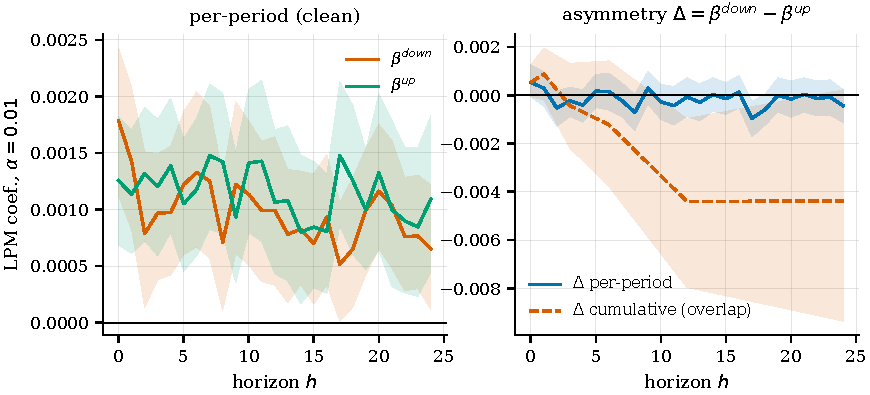
\includegraphics[width=\textwidth]{../paper/figures/fig5_exceedance_symmetry}
\caption{Per-period exceedance coefficients and paired asymmetry. Left: per-period exceedance coefficients at $\alpha = 1\%$, where both tails load positively. Right: the paired asymmetry $\Delta_h$ under the per-period construction (null everywhere) and under the overlapping cumulative construction (a significant asymmetry is manufactured at long horizons), the overlap artifact of Section~\ref{sec:overlap}.}
\label{fig:exceedance}
\end{figure}

An in-sample coefficient, however robust, is not yet a predictor. We use a
rolling-origin evaluation (weekly re-estimation, pinball loss on the
held-out tail forecasts, Diebold--Mariano inference on the loss
differentials \citep{diebold1995}). Adding the liquidation terms to an
otherwise identical quantile model improves tail forecasts directionally in
all twenty nested-QR cells, most not individually distinguishable from zero,
and significantly at both moderate tails at short horizons
(at one hour: \OosSkillFiveHone\% at $\tau = 0.05$,
$p = \OosPFiveHone$; \OosSkillNinetyFiveHone\% at $\tau = 0.95$,
$p = \OosPNinetyFiveHone$; Table~\ref{tab:oos}). These two cells, and a third at a long horizon ($\tau = 0.95$, twenty-four
hours), survive a Benjamini--Hochberg correction across the grid
($\OosNsurviveFDR$ of the twenty do, FDR-adjusted $p = \OosPFiveHoneFDR$ and $\OosPNinetyFiveHoneFDR$;
the 95\% cell survives even the stricter Holm bound), so the surviving
positive finding meets the multiple-testing discipline applied to the
interaction null. The symmetric reading carries out of sample. The boundary
is equally clear. Against a dedicated GARCH(1,1) scale benchmark the picture is deliberately
different: the augmented model does not systematically outperform it, the
short-horizon cells that beat the nested benchmark do \emph{not} beat GARCH
(one, $\tau = 0.95$ at one hour, significantly underperforms it), and the only
cells that beat GARCH are sparse long-horizon ones. That boundary is the point
rather than a concession. The liquidation signal is observable, predetermined, and
exogenous to any price model, so the information it carries is orthogonal and
incremental to the market-state controls a risk desk already tracks: a free
input to add to an existing tail-risk model, not a replacement for one.
Because pinball loss is the objective a quantile VaR forecaster minimizes,
the one-percent reduction at the moderate tails reads directly as a
calibration gain in a one-hour-ahead, on-chain-observable VaR signal,
consistent with the \citet{brownlees2021} finding that symmetric scale
models are formidable tail forecasters. A dollar quantification of that gain
would require position-level data and is left for future work.

\begin{table}[t]
\centering
\caption{Out-of-sample pinball skill of liquidation information (\%),
against a nested quantile benchmark (top panel) and a dedicated GARCH(1,1)
scale model (bottom panel).}
\label{tab:oos}
% GENERATED by scripts/paper/make_tables.py — DO NOT EDIT
% fragment only: wrap in \begin{table} + caption in the manuscript
\begin{tabular}{lccccc}
\toprule
 & $h=1$ & $h=3$ & $h=6$ & $h=12$ & $h=24$ \\
\midrule
\multicolumn{6}{l}{\emph{vs.\ nested QR (no liquidation terms)}} \\
$\tau=0.01$ & 1.41 & 1.03 & 1.10 & 1.18$^{*}$ & 0.81 \\
$\tau=0.05$ & 0.97$^{***}$ & 0.46$^{**}$ & 0.36$^{*}$ & 0.47$^{**}$ & 0.15 \\
$\tau=0.95$ & 0.85$^{***}$ & 0.56$^{**}$ & 0.37$^{*}$ & 0.26 & 0.60$^{***}$ \\
$\tau=0.99$ & 0.51 & 0.54 & 1.11$^{**}$ & 0.03 & 0.03 \\
\midrule
\multicolumn{6}{l}{\emph{vs.\ GARCH(1,1) benchmark}} \\
$\tau=0.01$ & 0.33 & -0.78 & 0.51 & 2.14$^{*}$ & 1.59 \\
$\tau=0.05$ & -0.61 & -0.61 & -0.16 & -0.19 & 1.00 \\
$\tau=0.95$ & -1.47$^{**}$ & -1.07 & -0.59 & -0.50 & 1.42$^{**}$ \\
$\tau=0.99$ & -0.44 & 0.41 & 1.38 & 0.29 & 2.51$^{*}$ \\
\bottomrule
\end{tabular}

\begin{minipage}{0.92\textwidth}
\vspace{2pt}
{\scriptsize \emph{Notes:} Rolling-origin forecasts of the per-period
$\tau$-quantile of ETH returns; expanding window, weekly refits, 97
re-estimations, $\sim$16{,}200 test hours. Skill $= 1 -
L_{\text{full}}/L_{\text{bench}}$ in percent; stars from Diebold--Mariano
tests with HAC variance ($^{*}$ $p<0.10$, $^{**}$ $p<0.05$, $^{***}$
$p<0.01$). Source: \texttt{oos\_predictive.csv}.}
\end{minipage}
\end{table}
\subsection{The bounded null}
\label{sec:boundednull}

Net of volatility, downside-specific
amplification is not economically significant, and what is excluded is
quantified in three steps.

\paragraph{(i) Raw symmetry.}
The paired asymmetry $\Delta_h = \beta^{\text{down}}_h -
\beta^{\text{up}}_h$, estimated on the same block resamples so the
difference is properly paired, is statistically indistinguishable from
zero at every horizon and tail level (Table~\ref{tab:nullbound}, Panel A):
at the 1\% level on impact, $\Delta_0 = \DeltaExcImpact$
($p = \DeltaExcImpactP$), with unstable signs across levels and horizons.

\paragraph{(ii) The standardized residual.}
Standardizing returns by predetermined volatility before forming the
asymmetry measures does not remove a scale bias. A symmetric scale
effect, predetermined or shock-induced, cancels in any down-minus-up
difference, which is why the raw paired contrast in (i) is already null.
What standardizing does is reduce the scale noise that masks a small shape
residual, raising power. At the moderate tail the residual is null
($p = \SkewTailFiveP$ at the 5\% level). At the extreme tail a small
positive residual becomes statistically detectable: $\beta = \SkewTailOne$ ($p = \SkewTailOneP$) on the 1\% tail
indicator, with a winsorized third-moment regression also significant
($\ZthreeWinsor$). This sharpening, not any new channel, is why the
residual surfaces here but not in the lower-powered raw contrast or in the
Section~\ref{sec:placebo} placebo, which compared the raw, vol-dominated
gap. Net of volatility, the extreme downside is therefore not
literally perfectly symmetric. The question that matters is whether
the detectable residual is large enough to matter.

\paragraph{(iii) The bound.}
It is not. Converting the bootstrap intervals into minimum detectable
effects and equivalence tests \citep{lakens2017,riesthuis2024} against the
pre-specified smallest effect size of interest
(Section~\ref{sec:method-battery}), the exceedance asymmetry at the 1\%
level is equivalent to negligible under all three calibrations of
the shock span, including the strictest (MDE at 80\% power
\MdeEightyExc{}, below the strictest SESOI of \SesoiStrict); the residual
itself is equivalent-to-negligible under two calibrations and borderline
under the strictest (Table~\ref{tab:nullbound}, Panel C, and
Figure~\ref{fig:mde}).\footnote{Read as a continuous function of the
smallest effect size rather than at the three pre-registered calibrations
alone, the verdict does not turn on the choice of span: the exceedance
$\Delta$ is equivalent-to-negligible for every SESOI above \SesoiEquivExc{},
at or below all three locked spans, so it clears even the strictest;
and the residual for every SESOI above \SesoiEquivSkew{}, which sits just
above the strictest span and hence above only it, leaving the strictest
calibration as the single inconclusive reading already noted.} The resulting
statement is the paper's central
quantitative claim: we can rule out a downside-specific tail
asymmetry larger than roughly \MdeEightyExc{} per unit of the log
liquidation shock, evidence of absence at the economically relevant
scale, not mere absence of evidence \citep{altman1995,ioannidis2017}. The moderate tails (5\%, 10\%) are underpowered for
strict equivalence, so the strong bound lives at the 1\% level. That is
also where the residual lives, so it is the bound that matters. The scope is narrow by design: the asymmetry the introduction documents is a far-extreme property, the $\pm 5\%$ and $\pm 7\%$ counts of Section~\ref{sec:stylized}, near the $0.1\%$ tail that an hourly panel cannot resolve, so the bound concerns one-percent-tail downside specificity rather than amplification of that far-extreme asymmetry. And the
third-moment regression is excluded from the equivalence exercise on
unit grounds (a third moment is not a probability gap).

\paragraph{The positive control.}
A bound is only as credible as the battery's ability to find what it
claims to exclude, so we ran the full equivalence apparatus on a synthetic
series into which a sign-specific downside cascade was planted at known
scale. The headline object behaves as a calibrated instrument
should: a planted asymmetry at half the smallest effect size of interest
is returned as equivalent-to-negligible and goes undetected (point
estimate \PosCtrlDeltaHalf{}); at the threshold itself the verdict is
inconclusive (\PosCtrlDeltaOne{}); and at twice the threshold the
asymmetry is recovered as non-negligible, its interval lying beyond the
band (\PosCtrlDeltaTwo{}). Because the standard error is a within-panel
block bootstrap anchored to the same \MdeEightyExc{} rather than to the
simulation budget, this graduation is a property of the data's information
content, not of how long we ran the planting. The equivalence apparatus
therefore detects a genuine, sign-specific downside asymmetry of
roughly twice \SesoiStrict{} and is correctly silent below it. That is
what converts the all-negative real result from ``we found nothing'' into
the sharper ``there is nothing at or above that scale to find.'' This certifies
the power of the equivalence apparatus, the object that claims the bound; the
symmetric placebo is deconstructive rather than a claim of absence and owes
no such demonstration, though the same planting also escapes its band at and
above that scale. One limit should
be stated. The cascade is planted in the units the tests read, so the
control certifies the battery's operating characteristics at a known,
now economically anchored, effect size rather than re-detecting a skew that
emerges from a structural process; a fully emergent cascade, a calibrated
leverage spiral, is left for future work.

\begin{table}[t]
\centering
\caption{Paired asymmetry, standardized skew, and equivalence verdicts.}
\label{tab:nullbound}
% GENERATED by scripts/paper/make_tables.py — DO NOT EDIT
% fragment only: wrap in \begin{table} + caption in the manuscript
\begin{tabular}{lcccc}
\toprule
\multicolumn{5}{l}{\emph{Panel A: paired exceedance asymmetry $\Delta_h = \beta^{\text{down}}_h - \beta^{\text{up}}_h$, $\alpha = 1\%$ (per-period)}} \\
$h$ & $\Delta$ & 95\% CI & & $p$ \\
\midrule
0 & 0.00053 & [-0.00006, 0.00125] & & 0.110 \\
1 & 0.00029 & [-0.00045, 0.00097] & & 0.428 \\
3 & -0.00023 & [-0.00088, 0.00033] & & 0.466 \\
6 & 0.00015 & [-0.00062, 0.00090] & & 0.694 \\
12 & -0.00007 & [-0.00087, 0.00072] & & 0.844 \\
24 & -0.00044 & [-0.00112, 0.00023] & & 0.234 \\
\midrule
\multicolumn{5}{l}{\emph{Panel B: vol-standardized skew tests (h=0)}} \\
measure & $\beta$ & 95\% CI & & $p$ \\
\midrule
tail indicator, $\tau{=}5\%$ & 0.00043 & [-0.00075, 0.00158] & & 0.446 \\
tail indicator, $\tau{=}1\%$ & 0.00071 & [0.00018, 0.00126] & & 0.012 \\
winsorised $z^3$ & -0.02930 & [-0.04391, -0.01479] & & $<$0.001 \\
\midrule
\multicolumn{5}{l}{\emph{Panel C: equivalence (TOST) verdicts vs.\ SESOI spans}} \\
object & MDE$_{80}$ & IQR span & strict span & $p_{10}{\to}p_{90}$ \\
\midrule
exceedance\_delta ($\alpha{=}$0.1 (h=0)) & 0.00231 & equiv. & inconcl. & inconcl. \\
exceedance\_delta ($\alpha{=}$0.05 (h=0)) & 0.00171 & equiv. & inconcl. & equiv. \\
exceedance\_delta ($\alpha{=}$0.01 (h=0)) & 0.00094 & equiv. & equiv. & equiv. \\
skew\_test (skew\_tail05) & 0.00166 & equiv. & inconcl. & equiv. \\
skew\_test (skew\_tail01) & 0.00077 & equiv. & inconcl. & equiv. \\
skew\_test (z3\_winsor) & 0.02081 & n/a & n/a & n/a \\
\bottomrule
\end{tabular}

\begin{minipage}{0.92\textwidth}
\vspace{2pt}
{\scriptsize \emph{Notes:} Panel A: paired moving-block bootstrap
($1{,}000$ replications, 24-hour blocks). Panel B: returns standardized by
predetermined 7-day realized volatility. Panel C: MDE at 80\% power and
TOST equivalence verdicts against the three SESOI calibrations of
Section~\ref{sec:method-battery}. Sources: \texttt{exceedance\_paired.csv},
\texttt{skew\_test.csv}, \texttt{mde\_equivalence.csv}.}
\end{minipage}
\end{table}

\begin{figure}[t]
\centering
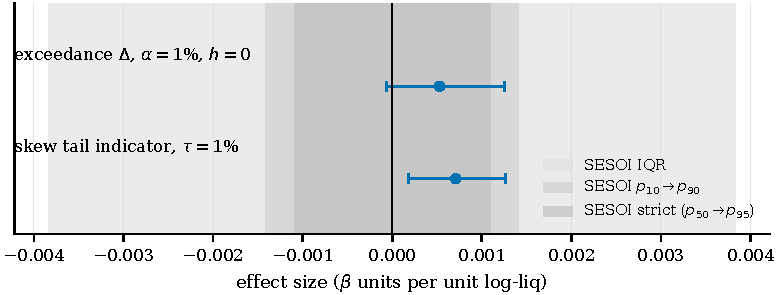
\includegraphics[width=\textwidth]{../paper/figures/fig7_mde_equivalence}
\caption{Point estimates and 95\% intervals for the two 1\%-tail asymmetry objects against the three SESOI bands. The residual is statistically detectable yet economically negligible.}
\label{fig:mde}
\end{figure}

\subsection{Stability}
\label{sec:stability}

The surviving objects are not the artifact of one episode or one tuning
choice. Splitting the sample in half leaves the tail profile essentially
unchanged. Excising the August 2024 episode, the largest liquidation
event in the sample, preserves about seventy percent of the
twelve-hour deepening ($\BetaQoneHtwelveLoo$ against \BetaQoneHtwelve)
while the paired asymmetry stays null in every subsample
(Table~\ref{tab:subsample}). The block-bootstrap inference, and hence the
equivalence bound itself, is insensitive to the block length: re-running
the critical cells at 12-, 36-, and 48-hour blocks moves the MDE by less
than a tenth of its value (Appendix Table~\ref{tab:blocksens}). One
sample nuance is reported. The small positive impact
tilt in $\Delta_0$ is concentrated in the first half of the sample
(2021--2023, the Terra/FTX era) and sits in the
contemporaneous-reverse-causality zone, vanishing at $h \ge 1$ and in the
later subsample.

\begin{table}[t]
\centering
\caption{Subsample stability: the tail profile and the paired asymmetry.}
\label{tab:subsample}
% GENERATED by scripts/paper/make_tables.py — DO NOT EDIT
% fragment only: wrap in \begin{table} + caption in the manuscript
\begin{tabular}{lcccccc}
\toprule
 & \multicolumn{4}{c}{$\beta_h(0.01)$} & \multicolumn{2}{c}{$\Delta$ at $h{=}12$} \\
\cmidrule(lr){2-5}\cmidrule(lr){6-7}
Subsample & $h=0$ & $h=6$ & $h=12$ & $h=24$ & estimate & MDE$_{80}$ \\
\midrule
Full sample & -0.032 & -0.160 & -0.241 & -0.213 & -0.00007 & 0.00112 \\
First half & -0.030 & -0.175 & -0.229 & -0.214 & -0.00005 & 0.00157 \\
Second half & -0.037 & -0.174 & -0.292 & -0.096 & 0.00017 & 0.00148 \\
Excl.\ Aug-2024 & -0.032 & -0.127 & -0.171 & -0.165 & -0.00002 & 0.00107 \\
\bottomrule
\end{tabular}

\begin{minipage}{0.92\textwidth}
\vspace{2pt}
{\scriptsize \emph{Notes:} $\beta_h(0.01)$ point estimates per subsample;
$\Delta$ at $h{=}12$ with its 80\%-power MDE from the paired bootstrap.
``Excl.\ Aug-2024'' drops a window around 2024-08-05 extended backward by
the maximal horizon, so the episode contaminates neither regressors nor
outcomes. Source: \texttt{subsample\_stability.csv}.}
\end{minipage}
\end{table}

\subsection{What we do not claim}
\label{sec:noclaim}

The guardrails. We do not claim that liquidations
\emph{cause} volatility or tail risk: at short horizons the relation is
bidirectional, and every estimate is a predictive association. We do not
claim the downside effect is literally zero: a 1\% residual is detectable;
we claim it is negligible and \emph{bounded}. Symmetrically, the residual
is not evidence of downside specificity: it is isolated (absent at the
5\% level and in the raw exceedance contrast), below the smallest effect
size of interest, and non-excluded rather than established. We do not
claim OECD-style elasticities, only sign and order of magnitude. And
we do not claim out-of-sample dominance over dedicated volatility models,
only incremental information. What we do claim is the conjunction:
a real, symmetric, bounded second-moment channel, validated in and out
of sample.